\begin{frame}
\frametitle{Implementazione Behavioural Covert Channel} 
Nel Behavioural Covert Channel implementato, l'evento 
sarà definito dall'arrivo di un messaggio ICMP. Il 
destinatario ricaverà il dato trasmesso osservando 
la tipologia di messaggio ed il codice presente per 
poi vedere a quale informazione è mappata la coppia.
\begin{figure}
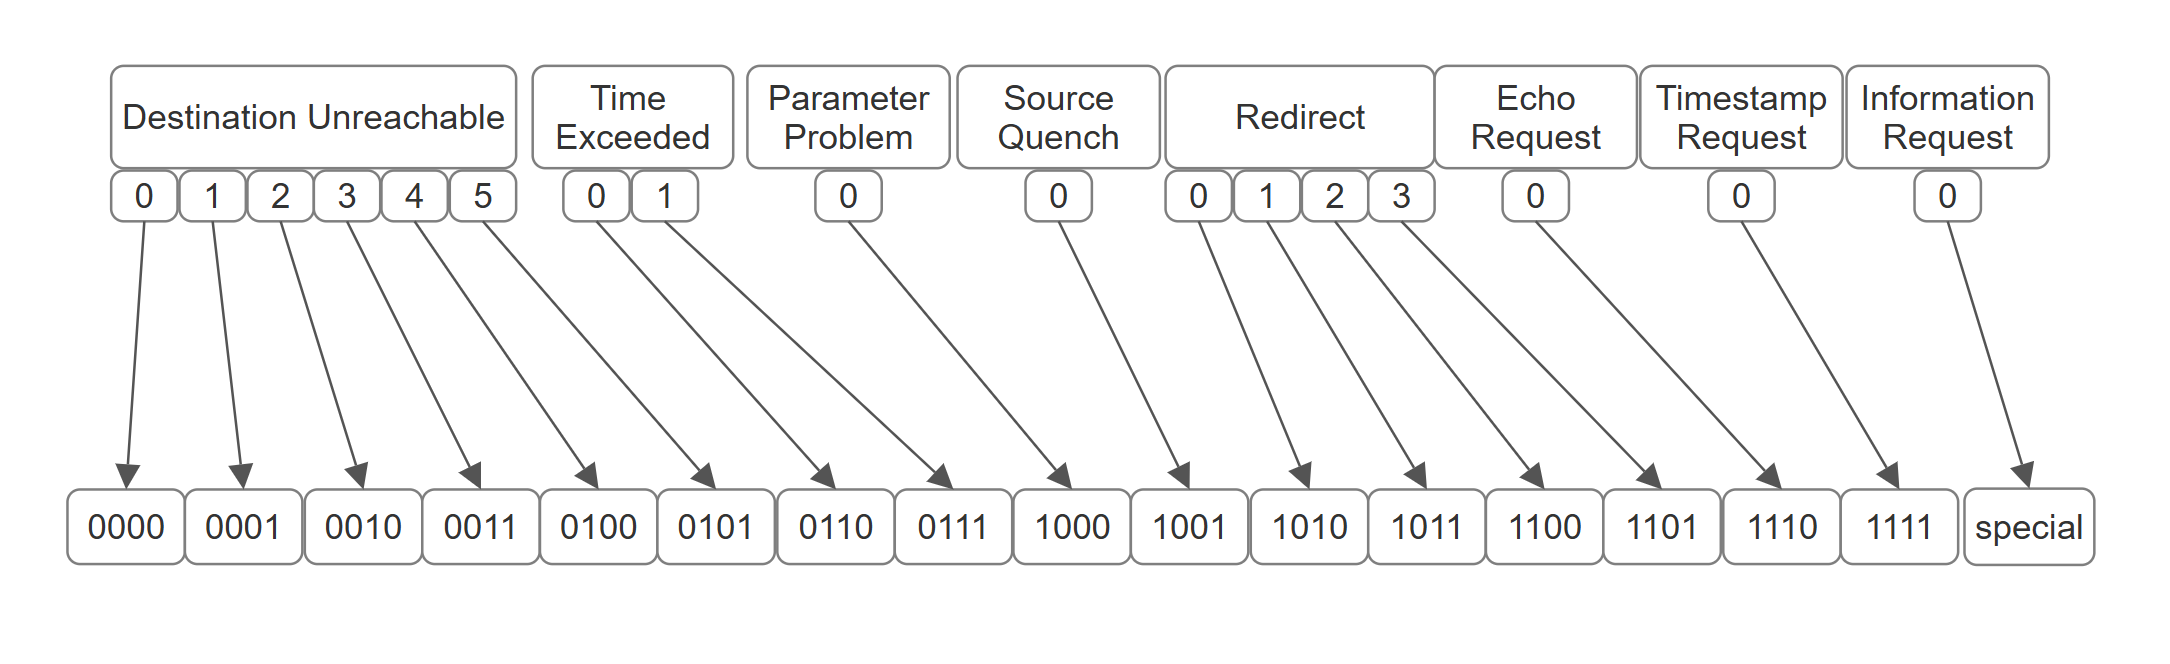
\includegraphics[width=\textwidth]{../Tesi/img/ICMP_behaveCC/behavioural_channel_1.png}
\end{figure} 
%\justifying 
Siccome il numero di eventi possibili sono 17, 
ognuno permetterà di codificare 4 bit alla volta 
($\log_216=4$). L'evento rimasto inutilizzato, 
verrà usato per indicare l'inizio e la terminazione 
dell'invio dei dati. 
\end{frame}
\begin{frame} [fragile] 
\scriptsize
\begin{lstlisting} 
data='m' 
data.hex=0x6D
data.bytes=b'0110 1101'

#PRIMO EVENTO 
Maschera il byte con b'11110000' per ottenere: 0x60 
Effettua lo shift a destra per ottenere: 0x06 (0110) 
Si ottiene come tipologia: Time Exceeded (tipo 11) 
Si ottiene come codice: 0 (Time to Live exceeded in Transit)
Invia un messaggio ICMP Time Exceeded con codice 0

#SECONDO EVENTO
Maschera il byte con b'00001111' per ottenere: 0x0D (1101) 
Si ottiene come tipologia: Redirect (tipo 5)
Si ottiene come codice: 3 (Redirect for the host)
Invia un messaggio ICMP Redirect con codice 3 
\end{lstlisting}
\captionof{lstlisting}{Esempio dell'invio di un byte} 
\end{frame} 

\begin{frame} [fragile]
\frametitle{Tipologie di messaggi deprecati}
Un problema di questa implementazione, sono 
le tipologie deprecate dei messaggi. Questi messaggi 
potranno comunque essere inviati ma le linee guida 
indicano ai router di ignorarli e all'host utente di 
non mandarli. 
\vspace{1ex} \newline 
L'uso di tipologie deprecate renderà il canale meno 
legittimo e maggiormente individuabile siccome il 
traffico sarà visto con sospetto. Infine date le linee 
guida, non è assicurata la ricezione dei messaggi. 
\scriptsize 
\begin{longtable}{|p{0.45\textwidth}|p{0.45\textwidth}|} 
    \hline 
    \textbf{Tipologia Messagio} & \textbf{Motivo} \\
    \hline  
    Information Request/Reply & è stato sostituito da 
    protocolli come il DHCP. \\  \hline  
    Source Quench & data la sua inefficenza, è stato 
    sostituito dai meccanismi presenti nel 
    protocollo TCP. \\ \hline 
    \caption{Tipologie di messaggi deprecati}  
\end{longtable} 
\end{frame}  
